\newpage
\subsection{Implementation of the embedded server}
This server can be implemented using any suitable hardware and software.
Choosed tools and libraries are not fixed and can be easily changed in
future.
Loosely coupled modules in the system give a possibility to change everything
without a need of global redesign.

The reason why technologies below are used is that they are simple to use and
easy to learn. They are also quite lightweight and therefore they can be used in
a embedded system.

\subsubsection{Hardware}
\label{sec:hardware}
\begin{center}
 \begin{figure}[h]
	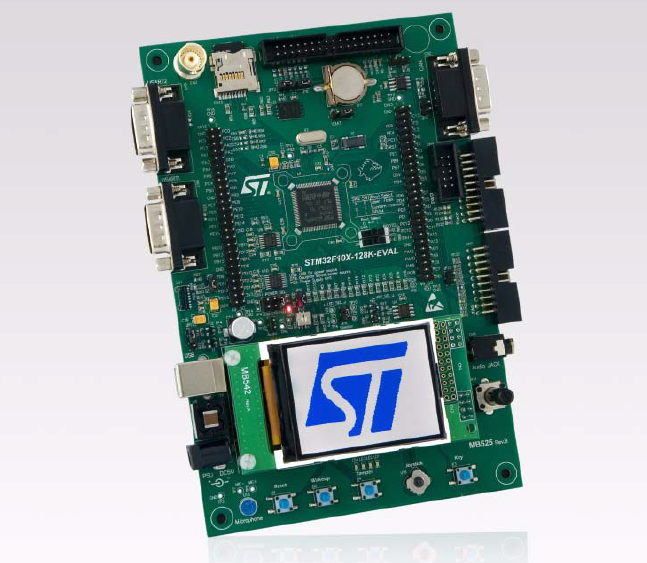
\includegraphics[width=\textwidth]{../images/implementation/embedded_server/stm3210b-eval.png}
	\caption{STM32F10X 128K evaluation board (STM3210B-EVAL)
	\cite{stm_eval_board_manual}}
	\label{fig:stm_eval_board}
 \end{figure}
\end{center}

The hardware used in this work are the two ARM Cortex M3 microcontrollers from
STMicroelectronics(\url{http://www.st.com/}). They were choosed because the
company already has a development board  and some other products from that
manufacturer. There is nothing special in that hardware and similar
microcontrollers from other manufacturers may be used in the same way.

The hardware features desribed below are common for almost all microcontrollers
and every well known manufacturer has similar device family.

Description will start from the first used STM32 microcontroller and
the STM3210B-EVAL evaluation board from STMicroelectronics.
These are features that this board has \cite{stm_eval_board_manual}:
\begin{itemize}
  \item Three 5V power supply options: power jack, USB connector or daughter
  board
  \item Boot from user Flash, test Flash or SRAM
  \item Audio play and record
  \item 64Mbyte MicroSD card
  \item Type A and Type B smartcard support
  \item 8Mbyte serial Flash
  \item I2C/SMBus compatible serial interface temperature sensor
  \item Two RS232 communication channels with support for RTS/CTS handshake on
  one channel
  \item IrDA transceiver
  \item USB 2.0 full speed connection
  \item CAN 2.0A/B compliant connection
  \item Induction motor control connector
  \item JTAG, SWD and trace tool support
  \item 240x320 TFT color LCD
  \item Joystick with 4-direction control and selector
  \item Reset, wakeup, tamper and user push buttons
  \item 4 LEDs
  \item RTC with backup battery
  \item Extension connector for daughter board or wrapping board 
\end{itemize}

As you see there are lots of opportunities to apply your creativity.
The amount of features is quite big, but we do not need most of them.
Required are only connectivity(RS232, USB) and debug(JTAG, SWD) interfaces.

This development board is made for evaluation of STM32F10x family
microcontrollers. These are ARM Cortex-M3 core-based mainstream microcontrollers
with a maximum CPU speed of 72 MHz and Flash memory amount from 16 Kbytes
to 1 Mbyte. They are equipped with large variety of peripherals.
\autoref{fig:stm32f103vbt6_hardware} covers interfaces of STM32F103VBT6 MCU that
is used in this board.

This controller is equipped with 20KB SRAM and 128KB Flash memory.
It has three USART transceivers and the debugging interface.
These are the main features we need.

\begin{center}
 \begin{figure}[h]
	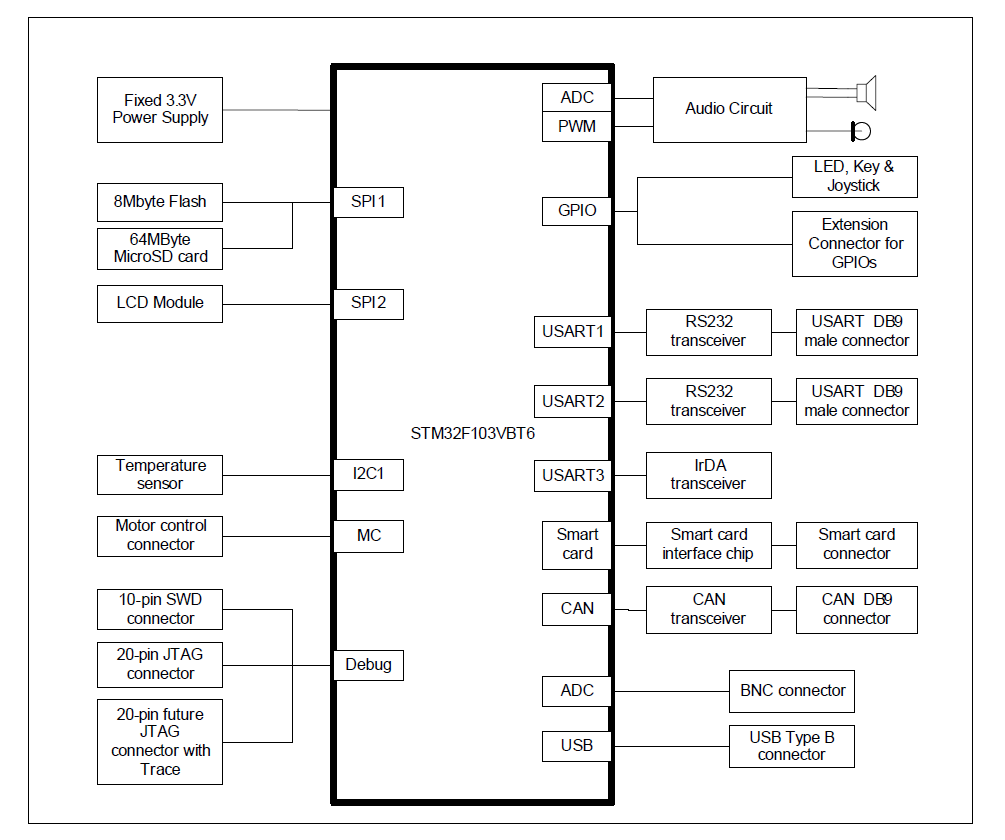
\includegraphics[width=\textwidth]{../images/implementation/embedded_server/stm32f103vbt6_hardware.png}
	\caption{Hardware block diagram of STM32F103VBT6 MCU on STM3210B-EVAL board
	\cite{stm_eval_board_manual}}
	\label{fig:stm32f103vbt6_hardware}
 \end{figure}
\end{center}

The second microcontroller that was used  is the STM32F103ZE MCU. It has more
memory:
64KB SRAM and 512KB Flash memory. This controller was choosed because the first
one has not enough resources, especially SRAM memory. The text messages, that
are transfered from client to server and back, require to be stored in the RAM
memory and each request has several copies of data while it is processed.
Amount of RAM on the first MCU was enough to execute optimized and final version of the server, but during development there is need for
storing additional debug information and to try different libraries.
The second reason is that service contracts are stored in the flash memory.
STM32F103VBT6 has 128 Kbytes of flash, however STM32F103ZE has 512 Kbytes.
System becomes more simple when service contract is stored together with
application code and there is no need to introduce another level of complexity (
connecting external storage device and programming connectivity code for
that). 


STM32F103ZE has 5 USART interfaces which is more than enough for this kind of
system. Three of them are used in the application: One for client-server
communication, one for logging and the third one for communicating with coffee
machine.

Client and server are connected using Bluetooth-to-serial module LMX9838 from
Texas Instruments.This module contains hardware and firmware support of
Bluetooth and Serial Port Profile and can be used as simple wireless serial
interface in communication between devices.

Server logging interface is connected to a personal computer using FTDI
Serial-to-USB chip (\url{http://www.ftdichip.com/}). This is popular solution of
connecting embedded systems and USB powered hardware. There is the virtual com
port on the PC side, that is powered by drivers of operating system. This
solution can be used instead of old serial connectors, that are not always
available on modern hardware.

Embedded service server and coffee machine are connected using serial line and
wires. This is a most simple connection here. Coffee machine has external serial
interface and STM32 microcontroller is connected directly to it.

That was a short overview of system hardware. Next comes description of system
software and operating system.

\subsubsection{Software and operating system}

\paragraph{Hardware configuration} ~\\
All MCU hardware is controlled by the software.
The execution of a trivial program (like "Hello world") on a
microcontroller requires a long list of instructions. To write some bytes to
UART or to blink with LED you usually need to:
\begin{enumerate}
  \item Configure MCU clock. Select clock source, frequency, clock prescalers
  \item Configure clock for peripheral buses. Again, the source and frequency by
  configuring prescalers. (Advanced Peripheral Bus in case of ARM)
  \item Turn on clocking for buses and peripherals.
  \item Configure general purpose input/output (GPIO) ports to use required
  function.
  \item Configure interrupt controller for the peripherals.
  \item In case of UART or any other communication, set the communication speed
  and configure the interface parameters.
  \item Write your application code
  \item Download the code to the device
  \item Debug the results
  \item Start from the beginning.
\end{enumerate}

Modern MCUs, especially with ARM Cortex-M architecture, have very complex
structure. They contain a huge amount of interfaces ( see \ref{sec:hardware}
section and feature list of evaluation board ) in a one single chip.
Most of peripherals are separately clocked, which gives a possibility to turn
off inactive ones and save the power energy. During MCU system startup
programmers code  should turn on and configure required peripheral modules.

In contrast, traditional software developing for desktop computers requires only
last four steps and the most complicated preparation step is the compiler and
IDE environment setup.

Each "configuring" step requires deep knowledge about what you are doing. MCU is
configured by values that are stored in memory mapped control registers. Each
register has a special purpose and different values written there configure
various MCU modules. In general words, you need to know these values to
configure the MCU system properly. Each bit in the control register represent
some setup setting.

Every controller family from various manufacturers differs from each other.
Therefore there is no need to write here in deep details how to configure one
special MCU named STM32F103ZE from STM32F1, what values to write into
\texttt{USART1->CR1} control register and which register bit turns on the UART
parity check. These instructions are not portable. When MCU hardware
changes(even families from a single manufacturer may highly differ) you need to
write this part once more.

There are two possible and more portable ways how to configure a STM32
microcontroller: Using CMSIS\footnote{The ARM® Cortex™ Microcontroller Software
Interface Standard (CMSIS) is a vendor-independent hardware abstraction layer for the Cortex-M processor series.}
from ARM and Standard Peripheral Library from STMicroelectronics. These are
hardware abstraction layer libraries that help to write portable code. They
define standard  application programming interace (API) for the ARM
architecture. Hardware vendors provide CMSIS compliant bindings for their
harware and programmers may write their code in standart manner, reducing
resources for platform change and reusing existing code.

Standard Peripheral Library is a C language library that provides standard API
for programming STM microcontrollers. It also contains CMSIS inside for
managing ARM core. There are several data structures, macros and functions that
help to configure and manage MCU peripherals.
The famous UART may be configured using Standard Peripheral Library like this:

\begin{listing}[H]
\begin{minted}[frame=lines,
               framesep=2mm]{c}
RCC_APB2PeriphClockCmd(RCC_APB2Periph_USART1, ENABLE);

USART_InitTypeDef USART_InitStructure;
USART_InitStructure.USART_BaudRate = 115200;
USART_InitStructure.USART_WordLength = USART_WordLength_8b;
USART_InitStructure.USART_StopBits = USART_StopBits_1;
USART_InitStructure.USART_Parity = USART_Parity_No;
USART_InitStructure.USART_HardwareFlowControl = USART_HardwareFlowControl_None;
USART_InitStructure.USART_Mode = USART_Mode_Rx | USART_Mode_Tx;
USART_Init(USART1, &USART_InitStructure);
\end{minted}
\caption{USART1 initialization using Standard Peripheral Library}
\label{lst:uart_init_example}
\end{listing} 

Most of configuration can be done using preprocessor defines.
You may add several defines, for example \texttt{#define STM32F10X_MD} to use
STM32 Medium density devices (Flash memory density ranges between 64 and 128
Kbytes). Clock rates and different peripherals can be adjusted in a similar way.

The distibution of STM Standard Peripheral Library contains a lot of
code and application examples, that helped me a lot. I have found there how to
configure a USART DMA\footnote{Direct Memory Access} controller and how to
transfer bytes using USART without intervention of central processing unit.
This is  quite good source for the begginers like me.

Setup an embedded development environment takes a lot of time and requires
deep knowledge about the underlying hardware. It is good to have such tools like
standart APIs, that help to make this process more easy.

\paragraph{Operating system}
Programs for embedded devices can be written in many different ways.
Some traditional ways how to do it:
\begin{itemize}
\item One big while loop and polling resources(also called busy waiting)
\item The same while loop, but it is interrupt driven.
Interrupts change some variables inside interrupt service routine (ISR) and main loop checks them on the next program cycle
\item The use of cooperative multitasking realtime operating system (RTOS) 
\end{itemize} 

The two first methods are often called bare metal approach.
Bare metal refers to techniques where programmers directly control and manipulate the underlying core, performing register-level access setting and clearing bits, and moving and operating on bytes of data directly.
Everything traces directly to the programmer’s next line of code being executed, and there is nothing in between the programmer and the hardware.
Resources like timers, interrupts, and I/O have to be accounted for in the application code.
The bare metal approach works well when a system has a  well defined and deterministic processing algorithm, only a couple of tasks to manage, or needs precise instruction level determinism(hard realtime).

Operating systems for microcontrollers have features like: 
multitasking/multithreading,task prioritization, interprocess communication, memory management, abstracted I/O drivers, file systems, networking.
They give to programmer higher level of abstraction and standard APIs, which help to reuse already existing code.
Popular RTOS already come with various protocol stack and drivers implementations.
However, the greates feature they have is the multitasking. 
The program could be divided into several separate tasks and these tasks could run in the parallel.
Parallel execution is achieved by dividing available CPU time between tasks.
This process is called \textit{scheduling}. 
There are two main scheduling policies: cooperative scheduling and preemptive scheduling.


During cooperative scheduling CPU time is used by a task until this task explicitly gives CPU time to other tasks.
This means that if the task will not give this time to others the whole system will hang.
This approach gives reliable and deterministic control over all tasks  and programmer needs to define CPU time release points.
There is no need of protection of common resources, because each task controls its execution and another task could run in that moment.

The second preemptive scheduling approach gives each task a regular "slice" of operating time. 
Each task has defined amount of CPU time during which it is able to do useful work.
Scheduler takes this time when this time is over and gives this to another task.
These tasks could have priorities, which allows to execute essential tasks before the backgroud are executed.
At the moment of the task context switch scheduled decides which task will be next according to the priority of available tasks.
Task with a higher priority will be triggered next. 
Scheduler should also be able to give the execution time to tasks with lower priorities, otherwise the will be never triggered because tasks with higher priorities will be lauched instead.
Tasks with the same priorities are executed one by one in the loop\cite{barry2010using}.
Such scheduling algorithm gives the illusion that tasks are running in parallel.
Parallel task execution requires protection of common and global hardware resources. 
For example, the situation when some task can change a global variable, while another task is reading it and makes some decision.
The result is that second task receives invalid result, which was modified between assigning a check value to some variable and reading it.


The coffee machine service application contains many different task like: 
multiple communication handling,
request processing,
request deserialization, etc.
This amount of tasks is not final.
This system needs to be extensible.
There should be an opportunity to add new request and communication handlers.
Request processing by the server is the concurrent process: while several requests are processed, another requests are sent over the network and communication interface needs to receive them.
Responce transmitting could also run in parallel.

It becomes harder to maintain and develop such concurrent program if you are not using a multitasking system. 
You need always to carefully think where to insert a functionality into a big polling loop.
Each insertion requires reordering of controll statements and checking the execution order of all parallell tasks.
Moreover, your application may handle two different independent tasks and you need to keep data separated and remember which task does each variable belong.
The use of operating system helps to keep things separated and loosely coupled.
 
\paragraph{FreeRTOS}
FreeRTOS is a popular real-time operating system for embedded devices, which has ports for many MCU devices(34 architectures \cite{FreeRTOS_website}), including STM32F1 family microcontrollers.
This operating system was choosed for the embedded service application implementaton in this work.
The reason is that this operating system has low entry level for the beginners and good documentation.
In addition to that i have found and read a book \cite{barry2010using}, which is a great introduction to FreeRTOS and embedded multitask systems programming. 

FreeRTOS has several features described below\cite{FreeRTOS_website}:
\begin{itemize}
\item Pre-emptive scheduling option 
\item Co-operative scheduling option
\item ROMable
\item 6K to 10K ROM footprint
\item Configurable / scalable
\item Compiler agnostic
\item Some ports never completely disable interrupts
\item Easy to use message passing
\item Round robin with time slicing
\item Mutexes with priority inheritance
\item Recursive mutexes
\item Binary and counting semaphores
\item Very efficient software timers
\item Easy to use API 
\end{itemize}

All this features and support of available hardware helped to make a choice of using FreeRTOS in this project.
I was inspired by this easy to use API, spread documentation and verbose examples.
Next i will describe some essential FreeRTOS APIs  and how tasks are created and managed.

The next thing you need to make after the setup of the programming environment and writing a trivial program to test it is the definition of system tasks.
A task in FreeRTOS is usual C function and \autoref{lst:freertos_task_function_prototype} contains a prototype of this function.


\begin{listing}[H]
\begin{minted}[frame=lines,
               framesep=2mm]{c}
void ATaskFunction( void *pvParameters );
\end{minted}
\caption{FreeRTOS task function prototype}
\label{lst:freertos_task_function_prototype}
\end{listing} 

Implementation of this function usually contains a separate program which has  infinite loop and never exits.  
Creation of temporary tasks which are finite is also possible.
Tasks may be deleted in the runtime using \texttt{vTaskDelete()} function.
Task function has no return type (void) and \texttt{return} statements are not allowed, they should be explicitly deleted.
It accepts method parameters of void pointer type, which allows to pass any type parameter there.
Required parameter needs to be casted to \texttt{void*} before passing the parameter.
It can be used inside task function through casting back to original type. 
This feature is used to pass a complex configuration structure to a system task in the embedded service design.

Task function do some useful application work. In order to start they require a registration in a system scheduler.
When microcontroller program first starts, it gets into reset interrupt service routine, where starts the hardware initialization process.
The \texttt{main()} application method is called after all hardware is initialized.
All tasks should be started in that \texttt{main()} application method, where the first application code usually starts.
\autoref{lst:freertos_task_create_function_prototype} shows task creation function prototype.
\begin{listing}[H]
\begin{minted}[frame=lines,
               framesep=2mm]{c}
portBASE_TYPE xTaskCreate( 
	pdTASK_CODE pvTaskCode, 
	const signed portCHAR * const pcName, 
	unsigned portSHORT usStackDepth, 
	void *pvParameters, 
	unsigned portBASE_TYPE uxPriority, 
	xTaskHandle *pxCreatedTask 
);
\end{minted}
\caption{FreeRTOS task function prototype}
\label{lst:freertos_task_function_prototype}
\end{listing} 

The first parameter is the pointer to a task function, which has the application logic.
Second parameter is the name of that task. It is used for system needs like debuging.
Parameter with name \texttt{usStackDepth} configures available stack space for the task.
Each context switch and method calls in a task use that memory space for storing application context.
Program counter and state of the operation registers are stored there.
All local variables are also copied to the stack during context switch.
Therefore this parameter should depend on the complexity of the application (function call depth) and
amount of local variables used in each child function. 
The fourth parameter is a pointer to the task parameters. Next parameter defines priority of that task.
The last one is the pointer to the task handle structure, which should be defined before this method call.
\texttt{xTaskCreate()} method returns a handle.  This handle may be used to control this task.

This method only creates  tasks, but not executes. 
\texttt{main()} application method should contain a \texttt{vTaskStartScheduler()} call, that executes the scheduler and registered tasks are executed by this scheduler.
\texttt{vTaskStartScheduler()} call is normally a blocking call, it never ends and runs until there is some error.


Freertos uses queues for interprocess communication.
This is an easy way of passing messages between tasks.

Listing of queue methods 
xQueueHandle xQueueCreate( unsigned portBASE_TYPE uxQueueLength, 
unsigned portBASE_TYPE uxItemSize 
); 

portBASE_TYPE xQueueSendToFront( xQueueHandle xQueue, 
const void * pvItemToQueue, 
portTickType xTicksToWait 
);

portBASE_TYPE xQueueSendToBack( xQueueHandle xQueue, 
const void * pvItemToQueue, 
portTickType xTicksToWait 
); 

portBASE_TYPE xQueueReceive( 
xQueueHandle xQueue,
const void * pvBuffer, 
portTickType xTicksToWait 
);

portBASE_TYPE xQueuePeek( 
xQueueHandle xQueue,
const void * pvBuffer, 
portTickType xTicksToWait 
);

Mutexes and semaphores
Semaphores and mutexes are base on queues and theid methods are similar to queue methods.



 





 

 – that relieve programmers from having to understand the underlying hardware in detail, and manage relatively complex tasks.
 Many of these tasks operate in the background without the programmer’s attention once the operating system starts.
 They work well in systems that need a lot of flexibility, and are generally for more sophisticated applications with larger code bases.
 Third party code is often available to help support features more quickly. 
 Faster processor clock speeds have blurred the lines on determinism somewhat, with most of these systems now fast enough for most applications. 
 Embedded versions of these platforms are usually configurable, so the footprint can be tuned by omitting unneeded resources from the build.


Why do we need an operating system to be installed on a 


\subsubsection{Service software}
Here will be STM32 server implementation.







%  One solution is to use closed encrypted proprietary
% protocol and be calm, but as it was mentioned earlier, it limits the possibility of integration
% between other embedded systems. It this case all of your devices should support
% that protocol and you choise of different hardware is limited. Proprietary
% protocols are often vendor-specific, code is closed, documentation is not free
% and all it works only with the proprietary devices from the manufacturer.
% 
% 
% \begin{center}
%  \begin{figure}[h]
% 	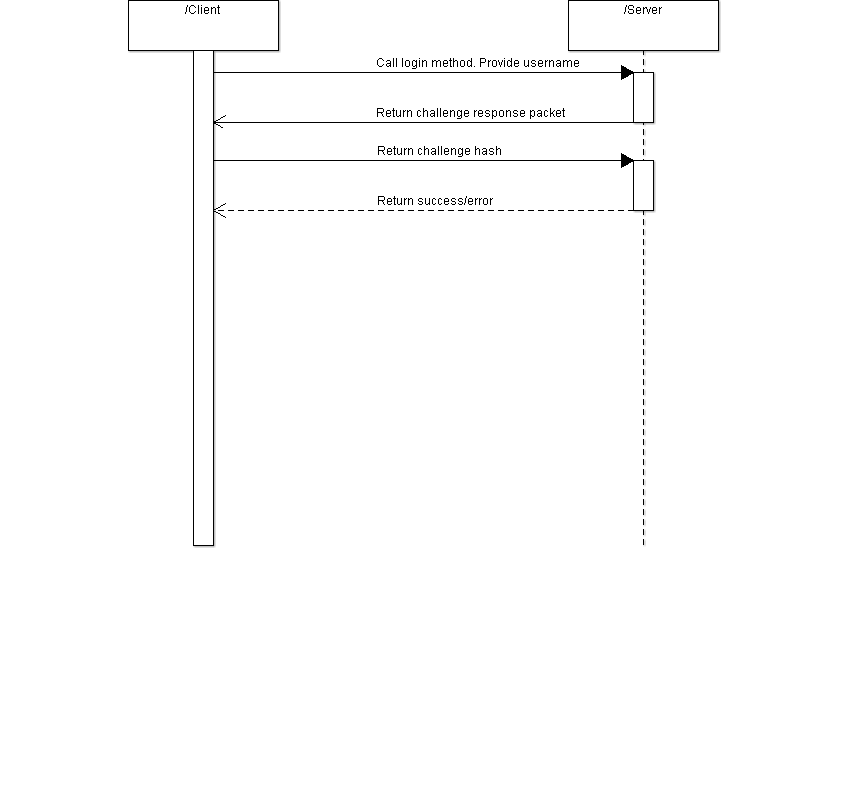
\includegraphics[width=\textwidth]{../images/implementation/embedded_server/SequenceDiagram.png}
% 	\caption{Client authentification process}
% 	\label{fig:embedded_server_login_auth}
%  \end{figure}
% \end{center}

%reversably encrypted form.

